\begin{markdown}

# Start: example\underscore md.tex

Das \ac{ABC} ist *toll* und **praktisch**.

* das ist eine
* Liste
    * mit
    * Unterliste

---

horizontal rulers work

> das ist ein blockquote
>
> mit break

## Chapter 1.1

lorem ipsum
\newline
\end{markdown} % lstlistings don't work properly from within markdown!
\begin{lstlisting}[language=sh,name={checking Nmap's version},label={sc:nmapversion}]
root::kali:MCS_WH1:# nmap -V | head -n1
Nmap version 7.91 ( https://nmap.org )
\end{lstlisting}
\begin{markdown}

lorem ipsum

\begin{figure}[!htbp]
\centering
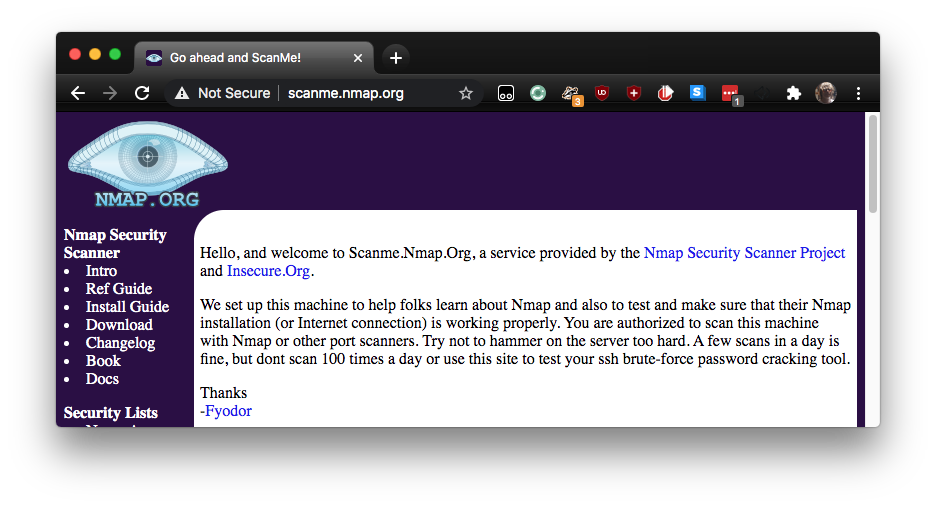
\includegraphics[width=1.05\linewidth]{media/scanme.nmap.org.png}
\caption{web server running at scanme.nmap.org}\label{webserver}
\end{figure}

Images work as well. See Figure \ref{sc:zahlenraten2}.
\newline
\end{markdown} % lstlistings don't work properly from within markdown!
\begin{lstlisting}[language={[x86masm]Assembler},name={disassembly of `zahlenraten`},label={sc:zahlenraten2}]
; ...
   0x0040077e <+14>:    56                  push   esi
   0x0040077f <+15>:    53                  push   ebx
   0x00400780 <+16>:    51                  push   ecx
=> 0x00400781 <+17>:    81 ec 08 02 00 00   sub    esp,0x2088
; ...
\end{lstlisting}
\begin{markdown}

Assembler Intel syntax works.

| left | mid | right |
| ---  | --- | ---   |
| left | mid | right |

: very descriptive table caption

% not sure how to link to those though..
\end{markdown}